%%%%%%%%%%%%%%%%
\section{Inner Controller}

\begin{frame}{Inner Controller}{}
    \uncover<1-3>{
    \begin{figure}[H]
        \centering
        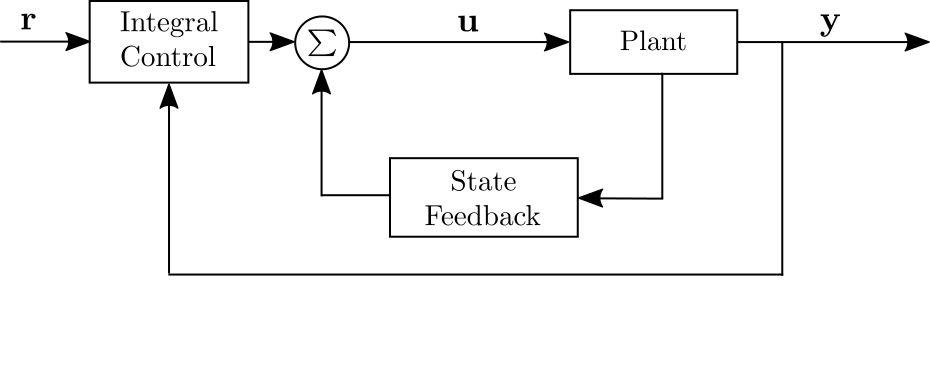
\includegraphics[width=0.6\linewidth]{figures/ControlDiagram}
    \end{figure}}
    \uncover<2-3>{
        \vspace{-0.3cm}
        \begin{itemize}
            \item Plant
        \end{itemize}
    \begin{figure}[H]
        \centering
        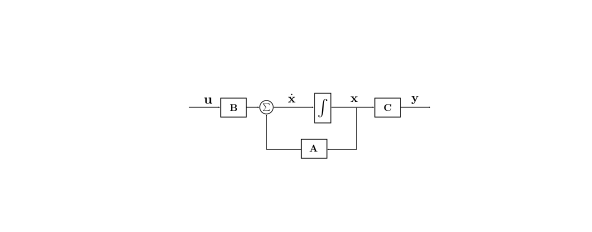
\includegraphics[width=0.45\linewidth]{figures/PlantSS}
    \end{figure}}
    \uncover<3>{
        \vspace{-0.3cm}
    \begin{itemize}
        \item Approaches
        \begin{itemize}
            \item $\mathcal{H}_\infty$ Controller
            \item Linear Quadratic Regulator
        \end{itemize}
    \end{itemize}}
\end{frame}

\begin{frame}{Inner Controller}{$\mathcal{H}_\infty$ Controller Design}
    \begin{itemize}
        \item Suboptimal $\mathcal{H}_\infty$ controller
    \end{itemize}
    \vspace{0.2cm}
    \begin{center}
        Find an internally stabilizing controller that provides a closed loop $\mathcal{H}_\infty$ norm less than some bound $\gamma$
    \end{center}
\end{frame}

\begin{frame}{Inner Controller}{$\mathcal{H}_\infty$ Controller Design}
    \begin{itemize}
        \item System structure
    \end{itemize}
    \begin{figure}[H]
        \centering
        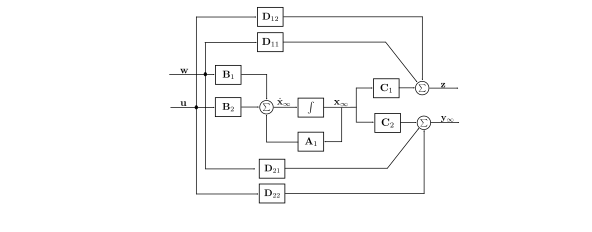
\includegraphics[width=0.55\linewidth]{figures/HinfDiag}
    \end{figure}
    \begin{minipage}[c][2.5cm]{\textwidth}
    \only<1|handout:1>{
    \begin{flalign}
    	\dot{\vec{x}}_\infty(t) &= \vec{A}_1 \vec{x}_\infty(t) + \vec{B}_1 \vec{w}(t) + \vec{B}_2 \vec{u}(t)\nonumber\\
    	\vec{z}(t) &= \vec{C}_1 \vec{x}_\infty(t) + \vec{D}_{11} \vec{w}(t) + \vec{D}_{12} \vec{u}(t)\nonumber\\
    	\vec{y}_\infty(t) &= \vec{C}_2 \vec{x}_\infty(t) + \vec{D}_{21} \vec{w}(t) + \vec{D}_{22} \vec{u}(t)\nonumber
    \end{flalign}}
    \only<2|handout:0>{
    \begin{flalign}	
    	\vec{u}(t) &= 
    	\begin{bmatrix}
    	F_1 & F_2 
    	\end{bmatrix}^\mathrm{T}\nonumber 
    \end{flalign}}
    \only<3|handout:0>{
    \begin{flalign}	
    	\vec{w}(t) &= 
    	\begin{bmatrix}
    	\psi_\mathrm{ref} & \dot{x}_\mathrm{b,ref} & F_\mathrm{wc} & \tau_\mathrm{wc} & F_\mathrm{wave} & \tau_\mathrm{wave}& n_{\psi} & n_{\dot{x}_\mathrm{b}}
    	\end{bmatrix}^\mathrm{T} \nonumber 
    \end{flalign}}
    \only<4|handout:0>{
    \begin{flalign}
    	\vec{y}_\infty(t) &= 
    	\begin{bmatrix}
    	\psi & \dot{x}_\mathrm{b} & \vec{x}_\mathrm{I}^\mathrm{T}
    	\end{bmatrix}^\mathrm{T}\nonumber 
    \end{flalign}}
    \only<5|handout:0>{
        \vspace{-0.55cm}
        \begin{flalign}
        \vec{x}_\infty(t) &=
        \begin{bmatrix}
        \psi & \dot{\psi} & \dot{x}_\mathrm{b} & x_{I_{\psi}} & x_{I_{\dot{x}_\mathrm{b}}} & x_{F_\mathrm{wc}} & x_{\tau_\mathrm{wc}} & x_{F_\mathrm{wave}} & x_{\tau_\mathrm{wave}} & x_{n_{\psi}}\ \ \  x_{n_{\dot{x}_\mathrm{b}}}
        \end{bmatrix}^\mathrm{T} \nonumber 
        \end{flalign}}
    \end{minipage}
\end{frame}

\begin{frame}{Inner Controller}{$\mathcal{H}_\infty$ Controller Design}
    \begin{itemize}
        \item Disturbance model
    \end{itemize}  
    \begin{figure}[H]
        \centering
        \includegraphics[width=0.6\linewidth]{figures/WeightDiag}
      \end{figure} 
      \begin{flalign}
      \frac{d'}{d}=\frac{a}{s+a} \rightarrow \dot{d}' = -a d' + a d \rightarrow \begin{cases} \dot{x}_\mathrm{d} = -a x_\mathrm{d} + a d \\ d' = x_\mathrm{d} \end{cases} \nonumber
      \end{flalign}    
\end{frame}
 
    
\begin{frame}<handout:0>{Inner Controller}{$\mathcal{H}_\infty$ Controller Design}
    \begin{itemize}
        \item System structure
    \end{itemize}
    \begin{figure}[H]
        \centering
        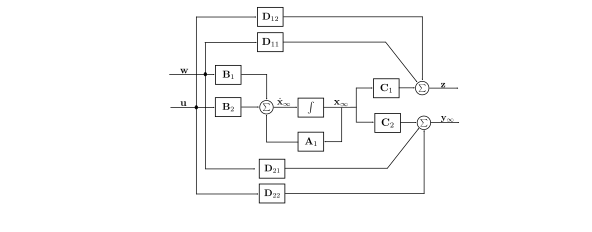
\includegraphics[width=0.55\linewidth]{figures/HinfDiag}
    \end{figure}
    \begin{minipage}[t][2.5cm]{\textwidth}
        \begin{flalign}	
        \vec{z}(t) &= 
        \begin{bmatrix}
        \vec{x}_\infty^\mathrm{T} & \vec{u}^\mathrm{T}
        \end{bmatrix}^\mathrm{T}\nonumber		
        \end{flalign}
    \end{minipage}
\end{frame}

\begin{frame}{Inner Controller}{$\mathcal{H}_\infty$ Controller Design}
    \begin{itemize}
        \item Controller design parameters ($\gamma$, $\vec{C}_1$, $\vec{D}_{12}$)
    \end{itemize}  
    \begin{minipage}{0.65\linewidth}
        \begin{flalign}
        \vec{C}_1 &=
        \begin{bmatrix}
            \vec{W}_\mathrm{x} & \vec{0}_{3\mathrm{x}2} &  \vec{0}_{3\mathrm{x}2} &  \vec{0}_{3\mathrm{x}2}  & \vec{0}_{3\mathrm{x}2} \\
            \vec{0}_{2\mathrm{x}3}  &  \vec{W}_\mathrm{I}  & \vec{0}_{2\mathrm{x}2} &  \vec{0}_{2\mathrm{x}2}  & \vec{0}_{2\mathrm{x}2} \\
            \vec{0}_{2\mathrm{x}3}  & \vec{0}_{2\mathrm{x}2} &  \vec{W}_\mathrm{wc} &  \vec{0}_{2\mathrm{x}2} &  \vec{0}_{2\mathrm{x}2} \\
            \vec{0}_{2\mathrm{x}3} &  \vec{0}_{2\mathrm{x}2}  & \vec{0}_{2\mathrm{x}2}  & \vec{W}_\mathrm{wave}  & \vec{0}_{2\mathrm{x}2} \\
            \vec{0}_{2\mathrm{x}3} &  \vec{0}_{2\mathrm{x}2}  & \vec{0}_{2\mathrm{x}2} &  \vec{0}_{2\mathrm{x}2} &  \vec{W}_\mathrm{noise} \\
            \vec{0}_{2\mathrm{x}3}  & \vec{0}_{2\mathrm{x}2}  & \vec{0}_{2\mathrm{x}2}  & \vec{0}_{2\mathrm{x}2} &  \vec{0}_{2\mathrm{x}2} \\
            \vec{0}_{2\mathrm{x}3}  & \vec{0}_{2\mathrm{x}2}  & \vec{0}_{2\mathrm{x}2}  & \vec{0}_{2\mathrm{x}2}  & \vec{0}_{2\mathrm{x}2} 
        \end{bmatrix}\nonumber
        \end{flalign} 
    \end{minipage}\hfill  
    \begin{minipage}{0.3\linewidth}
        \begin{flalign}
            \vec{D}_{12} &=
            \begin{bmatrix}
                \vec{0}_{2\mathrm{x}3} \\
                \vec{0}_{2\mathrm{x}2} \\
                \vec{0}_{2\mathrm{x}2} \\
                \vec{0}_{2\mathrm{x}2} \\
                \vec{0}_{2\mathrm{x}2} \\
                \vec{W}_\mathrm{u}
            \end{bmatrix} \nonumber
        \end{flalign}
    \end{minipage}\hfill 
 
\end{frame}


\begin{frame}{Inner Controller}{$\mathcal{H}_\infty$ Controller Design}
    \begin{itemize}
        \item Feedback gain
    \end{itemize}
    \begin{flalign}
        \vec{X}_\infty = Ric
        \begin{bmatrix}
        \vec{A}_1 & \gamma^{-2}\vec{B}_1\vec{B}_1^\mathrm{T} - \vec{B}_2\vec{B}_2^\mathrm{T} \\
        -\vec{C}_1^\mathrm{T}\vec{C}_1 & -\vec{A}_1^\mathrm{T}
        \end{bmatrix} \nonumber
    \end{flalign}
    \begin{flalign}
        \vec{F}_\infty = -\vec{B}_2^\mathrm{T}\vec{X}_\infty \nonumber
    \end{flalign}
\end{frame}
